\documentclass[review]{elsarticle}

\usepackage{lineno,hyperref}
\usepackage{pdflscape}
\modulolinenumbers[5]

\journal{Geochemica and Cosmochemica Acta}

%%%%%%%%%%%%%%%%%%%%%%%
%% Elsevier bibliography styles
%%%%%%%%%%%%%%%%%%%%%%%
%% To change the style, put a % in front of the second line of the current style and
%% remove the % from the second line of the style you would like to use.
%%%%%%%%%%%%%%%%%%%%%%%

%% Numbered
%\bibliographystyle{model1-num-names}

%% Numbered without titles
%\bibliographystyle{model1a-num-names}

%% Harvard
\bibliographystyle{model2-names.bst}\biboptions{authoryear}

%% Vancouver numbered
%\usepackage{numcompress}\bibliographystyle{model3-num-names}

%% Vancouver name/year
%\usepackage{numcompress}\bibliographystyle{model4-names}\biboptions{authoryear}

%% APA style
%\bibliographystyle{model5-names}\biboptions{authoryear}

%% AMA style
%\usepackage{numcompress}\bibliographystyle{model6-num-names}

%% `Elsevier LaTeX' style
%\bibliographystyle{elsarticle-num}
%%%%%%%%%%%%%%%%%%%%%%%

\begin{document}

\begin{frontmatter}

\title{Modelling excess properties of mineral and melt solutions over large P-T ranges: implications for phase relations and seismic velocities in the mantle}
%\tnotetext[mytitlenote]{Fully documented templates are available in the elsarticle package on \href{http://www.ctan.org/tex-archive/macros/latex/contrib/elsarticle}{CTAN}.}

%% Group authors per affiliation:
\author{R. Myhill}
\address{Bayerisches Geoinstitut, Universit\"{a}t Bayreuth, Universit\"{a}tsstrasse 30, 95447 Bayreuth, Germany}
\cortext[mycorrespondingauthor]{Corresponding author: R. Myhill}
\ead{myhill.bob@gmail.com}

\begin{abstract}
  Thermodynamic models of solid and liquid solutions in the Earth Sciences are increasingly used to calculate phase relations and seismic properties over large pressure and temperature ranges. Calculations often span over 1000 K and 5 GPa in studies of exhumation processes and metamorphism in subduction zones. Research into mantle phase relations and differentiation of the early Earth frequently involves calculations over 3000 K and 100 GPa. Despite spanning such huge ranges, a common approximation is that excess thermodynamic derivatives within solid solutions (entropy and volume) are pressure-temperature invariant. If these excesses are large, the approximation can result in large errors in gibbs free energy at high pressure and temperature, and errors in seismic velocities even within the range of calibration conditions. 

  In this paper, we present a solution to this problem by extending the subregular Margules mixing model using intermediate compounds to define the thermodynamic properties of solid solutions. Mathematical derivations are provided for excess properties ($H^{ex}$, $S^{ex}$, $V^{ex}$) and their pressure and temperature derivatives ($K_T^{ex}$, $\alpha^{ex}$, $Cp^{ex}$ etc.). We provide examples of pyroxene, garnet and melt solutions, showing that inclusion of a variable excess volume is vital to simulate observed phase relations and seismic velocities. Heuristics are suggested for intermediate compounds where individual thermodynamic properties are poorly constrained.


\end{abstract}

\begin{keyword}
high pressure \sep excess properties
\end{keyword}

\end{frontmatter}

\linenumbers

\section{Introduction}

Thermodynamic models of solid and liquid solutions in the Earth Sciences are an integral part of 


  The approximation of constant positive excess volume implicitly yields an excess positive bulk modulus and negative thermal expansion, in conflict with both intuition and experimental observations. This is a particular problem where thermodynamic data are used over pressure ranges exceeding a few GPa, and where they are used to compute seismic wave velocities. 

In many circumstances, these shortcomings are unimportant. However, there is a fundamental need to adjust the solid solution model where the stability range of the solid solution extends over pressure regimes large enough to contribute significantly to changes in excess enthalpy inconsistent with data, or mineral phases exhibit significant excess bulk moduli. The latter is especially important for those studies where velocities are obtained from the models.

The models in this study are all implemented in the open software \emph{burnman}, a mineral physics toolkit written in python. The software, first described in \cite{CHRU2014}, was originally designed for seismic velocity calculations. It has since been augmented with thermodynamics functionality, including a range of different models for solid solutions.

\section{The Extended Subregular Margules (ESM) model}
The subregular Margules mixing model within a binary system approximates excess Gibbs free energies at any given pressure and temperature as a cubic function of composition \citep{HW1989}:
\begin{equation}
  \mathcal{G}^{xs} = W_{12} X_1X_2^2 + W_{21} X_1^2X_2 
\end{equation}
The terms $W_{ij}$ describing the interaction between endmembers $i$ and $j$ are normally described by a function of the form
\begin{equation}
  W_{ij} = a_{ij} + b_{ij}P + c_{ij}T
\end{equation}
dropbox
In the ESM model, we instead define properties for each binary pair based on two intermediate compounds with compositions $X_i = X_j = 0.5$. For the special case of a symmetric mixing model, the properties for both intermediates are the properties of a compound with that composition; otherwise, both compounds are fictional. The interaction terms are now defined as:

\begin{equation}
  W^{\mathcal{G}}_{ij} = 4(\mathcal{G}_{ij} + T\mathcal{S}^{\textrm{conf}}_{ij}) - 2(\mathcal{G}_i + \mathcal{G}_j)
\end{equation}

\noindent where $\mathcal{S}^{\textrm{conf}}_{ij}$ is the configurational entropy of the intermediate compound, which depends on the number of sites on which mixing occurs. For a solution with $n$ independent endmembers, and ignoring ternary terms, the excess nonconfigurational Gibbs free energy is \citep{HW1989} 

\begin{equation}
  \mathcal{G}^{xs} = \sum_{i=1}^n \sum_{j>1}^n X_i X_j \left ( W_{ij} X_j + W_{ji} X_i + 0.5 (W_{ij} + W_{ji}) \sum_k^n (1-\delta_{ik})(1-\delta_{jk}) X_k \right)
  \label{xs}
\end{equation}

Using this new model, we can now define the properties of the solid solution as follows:

\begin{eqnarray}
\mathcal{G} = \sum_i X_i \mathcal{G}_i + \mathcal{G}^{xs} \\
\mathcal{H} = \sum_i X_i \mathcal{H}_i + \mathcal{H}^{xs} \\
\mathcal{S} = \sum_i X_i \mathcal{S}_i + \mathcal{S}^{xs} \\
\mathcal{V} = \sum_i X_i \mathcal{V}_i + \mathcal{V}^{xs} \\
C_P = \sum_i X_i C_P  + T \left( \frac{\partial \mathcal{S}}{\partial T} \right)_P^{xs} \\
\alpha = \frac{1}{\mathcal{V}} \left ( \sum_i X_i \alpha_i \mathcal{V}_i + \left( \frac{\partial \mathcal{V}}{\partial T} \right)_P^{xs} \right) \label{alpha} \\
K_T = \frac{\mathcal{V}}{\sum_i \frac{X_i \mathcal{V}_i }{K_{Ti}} - \left( \frac{\partial \mathcal{V}}{\partial P} \right)_T^{xs} } \label{K_T} \\
C_V = C_P - \mathcal{V} T \alpha^2 K_T \\
K_S = K_T \frac{C_P}{C_V} \\
\gamma = \frac{\alpha K_T \mathcal{V}}{C_V}   
\end{eqnarray}

With the exception of the enthalpy excess, excess terms ($\mathcal{S}^{xs}$, $\mathcal{V}^{xs}$ etc) are derived in the same way as the excess Gibbs free energy (Equation \ref{xs}), with interaction terms defined as follows:

\begin{eqnarray}
  W^{\mathcal{S}}_{ij} = 4 (\mathcal{S}_{ij} - \mathcal{S}^{\textrm{conf}}_{ij}) - 2(\mathcal{S}_i + \mathcal{S}_j) \\
  W^{\mathcal{V}}_{ij} = 4 \mathcal{V}_{ij} - 2(\mathcal{V}_i + \mathcal{V}_j) \\
  W^{\partial\mathcal{V}/\partial P}_{ij} = -4 \mathcal{V}_{ij}/K_{T{ij}} + 2(\mathcal{V}_{i}/K_{T{i}} + \mathcal{V}_{j}/K_{T{j}}) \\
  W^{\partial\mathcal{V}/\partial T}_{ij} = 4 \alpha_{ij} \mathcal{V}_{ij} - 2(\alpha_{i} \mathcal{V}_i + \alpha_{j} \mathcal{V}_j) \\
  W^{\partial\mathcal{S}/\partial T}_{ij} = \frac{4 C_{P{ij}} - 2(C_{P{i}} + C_{P{j}})}{T} 
\end{eqnarray}

Finally, excess enthalpy is defined as
\begin{equation}
 \mathcal{H}^{xs} = \mathcal{G}^{xs} + T\mathcal{S}^{xs}
\end{equation}

\subsection{Heuristics}
It is often the case that endmembers are particularly well studied, while the properties of the solid solution are constrained only by enthalpies of solution and volumes at room temperature and pressure. In the absence of other data, heuristics are required to constrain the properties of the intermediate compounds. In this study, we suggest that the following heuristics be used:
\begin{eqnarray}
  \mathcal{S}_{ij} = 0.5(\mathcal{S}_i + \mathcal{S}_j) + \mathcal{S}^{\textrm{conf}}_{ij} \\
  C_{P{ij}} = 0.5(C_{P{i}} + C_{P{j}}) \\
  \alpha_{ij} = 0.5 \mathcal{V} \left(\frac{\alpha_i}{\mathcal{V}_i} + \frac{\alpha_j}{\mathcal{V}_j}\right)\\
  K'_{T} = -\frac{\partial}{\partial P} \left (\mathcal{V}\left( \frac{\partial P}{\partial \mathcal{V}} \right)_T \right) \sim \mathcal{V} \left(\sum_i \frac{X_i \mathcal{V}_i}{K'_{Ti} + 1} \right)^{-1} - 1
\end{eqnarray}

If excess volumes are zero, the bulk modulus is given by Equation \ref{K_T}, with the differential term equal to zero. However, non-zero excess volumes are unlikely to remain constant with pressure and temperature. Mixing of elements with different ionic radii and chemical bonding on sites affects not only the packing efficiency, but also the mechanisms of compression. A positive excess volume implies a more open structure which will be more prone to volume decrease on compression.

We suggest that, in the absence of other data it should be assumed that $\left( \frac{\partial \mathcal{V}}{\partial P} \right)_T^{xs} \rightarrow 0$ as $P \rightarrow \infty$. Bulk moduli for intermediates can then be constrained. 

\begin{equation}
  K_{T} \sim 0.5(K_{Ti} + K_{Tj}) + c \left(\frac{K_{Ti}\mathcal{V}_{j} + K_{Tj}\mathcal{V}_{j}}{\mathcal{V}_{i} + \mathcal{V}_{j}} - 0.5(K_{Ti} + K_{Tj})\right)
  \label{K_T_heuristic}
\end{equation}

The factor $c$ before the second term on the RHS of Equation \ref{K_T_heuristic} modifies the rule of thumb proposed by \cite{AA1970} to estimate the compressibility of endmembers based on their molar volumes. Typically, values of $c$ from 4 to 12 satisfy our proposed heuristic.

\section{Examples}
\subsection{Pyroxene}
Our first example is that of jadeite-aegirine pyroxene, an almost ideal solid solution (from a volumetric perspective). We use this model to illustrate that even when excess volumes are extremely small, excess bulk moduli are resolvable. The experimental data is that of \cite{NBLBT2006}, and the equation of state used is the Modified Tait \citep{HP2011}. The fit to the volume data is shown in Figure \ref{fig:PV_jadeite_aegirine}.

\begin{figure}[ht!]
  \centering
  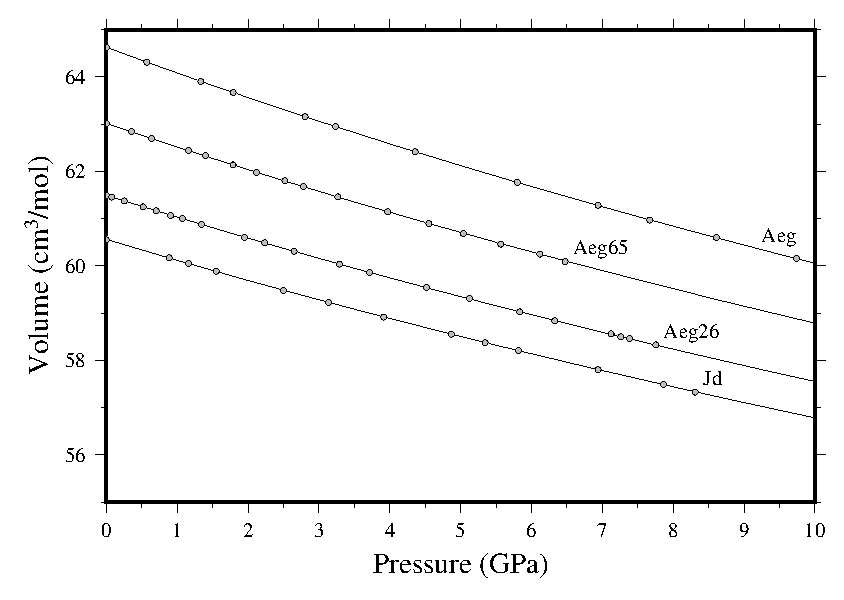
\includegraphics[width=0.8\textwidth]{figures/jadeite_aegirine_P_V}
  \caption{Pressure-volume data in the binary system Jadeite-Aegirine \citep{NBLBT2006}, with the model proposed in this study.}
  \label{fig:PV_jadeite_aegirine}
\end{figure}

\begin{table}[]
\centering
\caption{Jadeite-Aegirine mixing parameters to fit the room temperature data of \cite{NBLBT2006}. The value for $K'_0$ is fixed to the value given by the heuristic proposed in the text. $K''_0 = -K'_0/K_0$.}
\label{tab:jd_aeg}
\begin{tabular}{lllll}
                   & jadeite              & aegirine             & jd50ae50             & ae50jd50             \\
$V_0$ (cm$^3$/mol) & 60.5640 $\pm$ 0.0001 & 64.6261 $\pm$ 0.0004 & 62.3641 $\pm$ 0.0005 & 62.4522 $\pm$ 0.0005 \\
$K_0$ (GPa)        & 133.5 $\pm$ 0.2      & 116.0 $\pm$ 0.2      & 124.8 $\pm$ 0.5      & 126.7 $\pm$ 0.4      \\
$K'_0$             & 4.6                  & 4.4                  & 4.4785               & 4.4785              
\end{tabular}
\end{table}

Using the derived properties of the solid solution, we can fit the excess volume as a function of pressure (Figure \ref{fig:excess_volume_jadeite_aegirine}). The decay of excess volume as a function of pressure is in excellent agreement with the heuristic proposed in the previous section.

\begin{figure}[ht!]
  \centering
  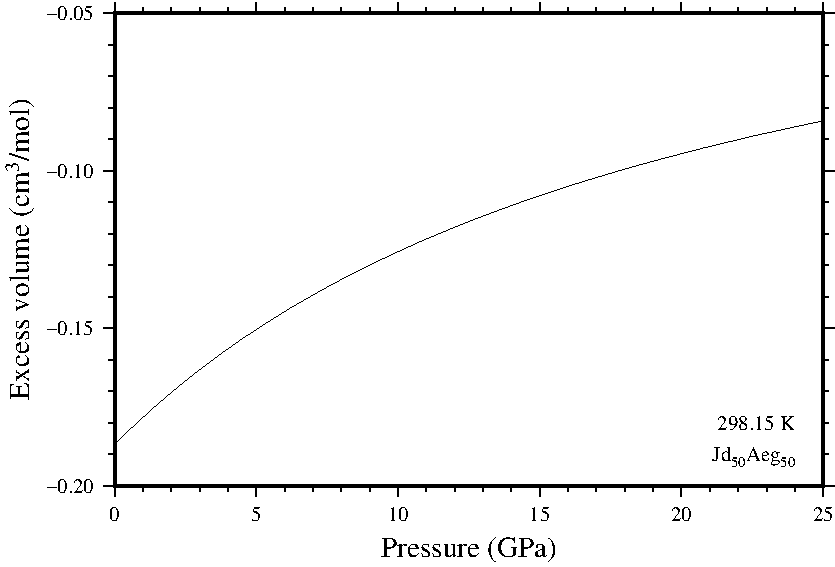
\includegraphics[width=0.8\textwidth]{figures/jadeite50aegirine50_Vex}
  \caption{Excess volume for Jd$_{50}$Aeg$_{50}$ calculated from our model.}
  \label{fig:excess_volume_jadeite_aegirine}
\end{figure}

\subsection{Garnet}
Our second example is the pyrope-grossular join, which is well-known to have significant non-ideality and volumes of mixing. Here we use the excess volume of \cite{DCW2015}, approximating the solid solution as symmetric and using the heuristics described above.

\begin{figure}[ht!]
  \centering
  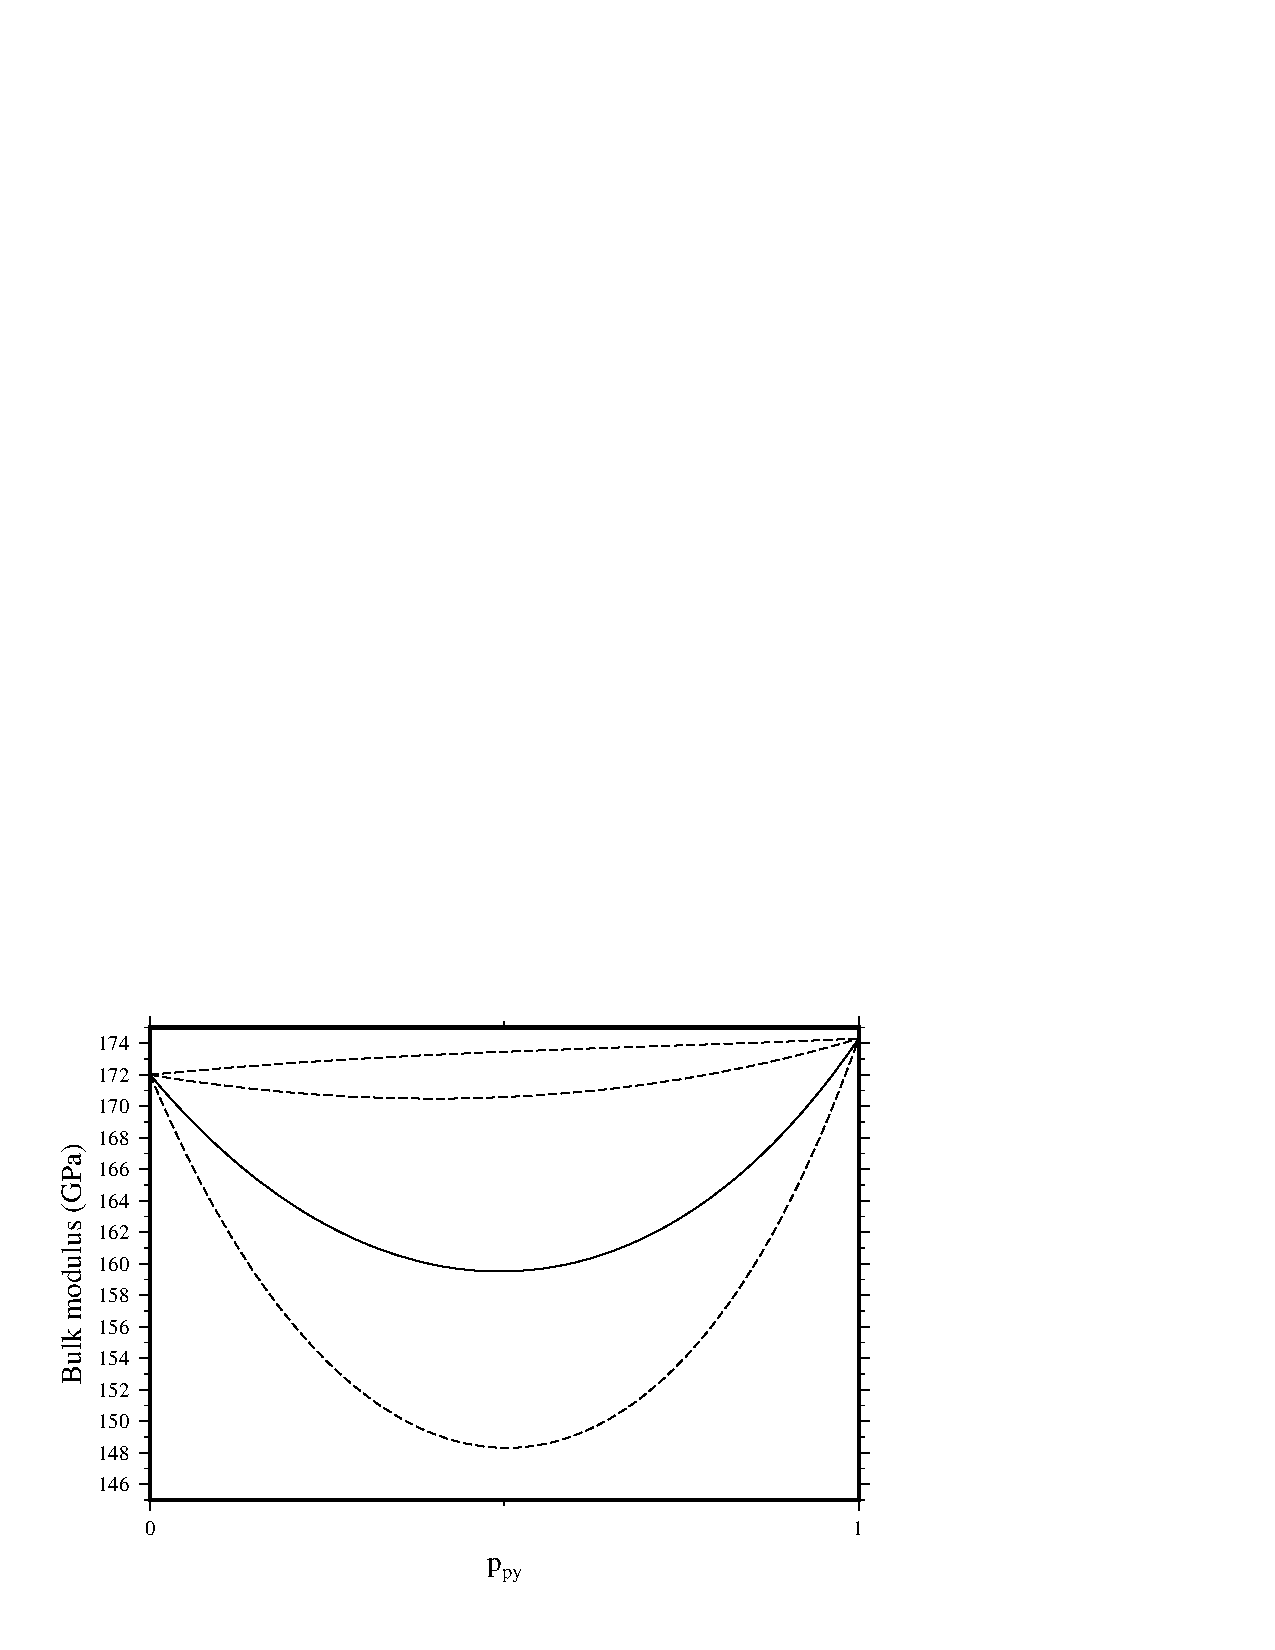
\includegraphics[width=0.8\textwidth]{figures/pyrope_grossular_P_V}
  \caption{Pressure-volume data in the binary system Pyrope-Grossular \citep{DCW2015}, with the model proposed in this study.}
  \label{fig:PV_pyrope_grossular}
\end{figure}


P-wave , S-wave and bulk sound velocities are functions of isentropic bulk and shear moduli and density:
\begin{eqnarray}
V_P = \sqrt \frac{K_S + \frac{4}{3} G }{\rho} \\
V_S = \sqrt \frac{G}{\rho} \\
V_\Phi = \sqrt \frac{K_S}{\rho}
\end{eqnarray}
To illustrate the effect of excess bulk moduli on seismic wave velocities, we plot $V_\Phi$ for a 50:50 molar mix of pyrope and grossular according to three solid solution models (Figure \ref{fig:bulk_sound_garnet}).

\begin{figure}[ht!]
  \centering
  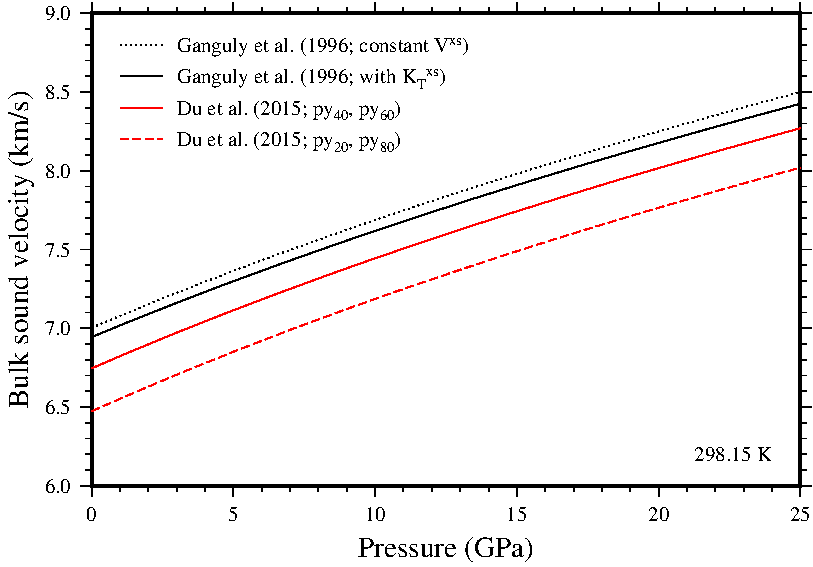
\includegraphics[width=0.8\textwidth]{figures/pyrope_grossular_bulk_sound_velocities}
  \caption{Bulk sound velocities of Py$_{50}$Gr$_{50}$ at room temperature according to the model of \citep{GCT1996}, a fixed excess volume based on room pressure data \citep{DCW2015} and a full subregular model incorporating excess bulk moduli, from the same study.}
  \label{fig:bulk_sound_garnet}
\end{figure}

We note that for natural garnet, $(\partial \ln V_S / \partial \ln V_P)_P \sim 1$ \citep{CBS1997}, and therefore $V_p/V_S \sim c$ with varying temperature. With this in mind, $V_P$ and $V_S$ should be constant fractions of the bulk sound velocity $V_\Phi$.
\subsection{Fe-O melt}

Our final example is that of Fe-FeO melt. This liquid solution is extremely important for understanding partitioning of oxygen into the Earth's core. At pressures $<$25 GPa, the solution exhibits signficant non-ideality, with a large miscibility gap between ionic and metallic Fe-O liquids \citep{Frostetal2010}. As pressure increases, this miscibility gap disappears, indicating a negative excess volume of mixing (Figure \ref{fig:Fe_O_solvus}). \cite{Kom2014} uses an ideal model at high pressure, and obtains a more-or-less reasonable fit to the available experimental data. 

To model processes of mantle differentiation and core formation, it would be extremely useful to have a single model describing the properties of melts over relevant pressure and temperature ranges. Clearly a high pressure ideal model cannot be reconciled with a low pressure model with large excess volumes of mixing without incorporating excess bulk moduli and thermal expansivities. Here, we use the compositions of coexisting metallic and ionic liquid \citep{} and the pressure, temperature and compositions of eutectic liquid at high pressure \citep{} to constrain the mixing properties of Fe-FeO liquid (Figure \ref{fig:Fe_O_interaction}). The eutectic temperature and composition above 25 GPa are shown in Figure \ref{fig:Fe_O_melting}.

\begin{figure}[ht!]
  \centering
  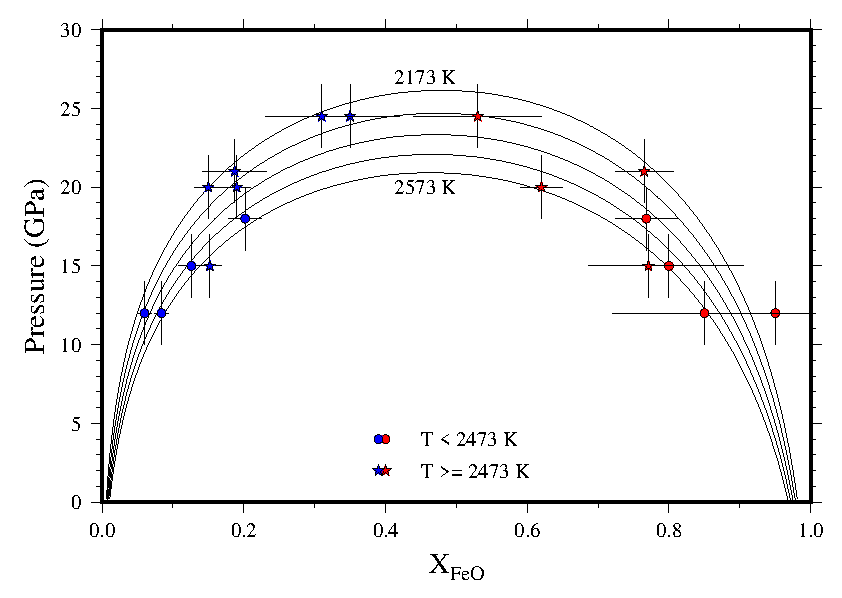
\includegraphics[width=0.8\textwidth]{figures/Fe_FeO_solvus}
  \caption{Fe-O solvus}
  \label{fig:Fe_O_solvus}
\end{figure}

\begin{figure}[ht!]
  \centering
  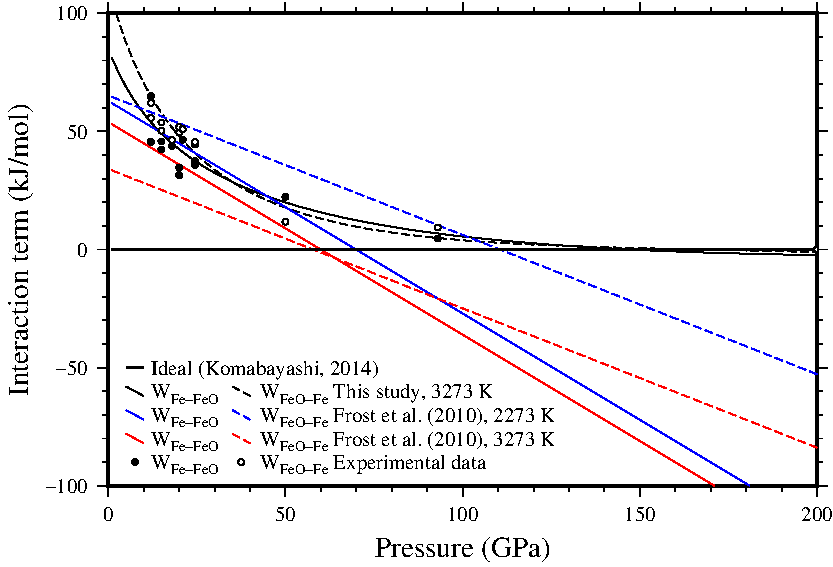
\includegraphics[width=0.8\textwidth]{figures/Fe_FeO_interaction_terms}
  \caption{Interaction terms in Fe-FeO melt as a function of pressure.}
  \label{fig:Fe_O_interaction}
\end{figure}

\begin{figure}[ht!]
  \centering
  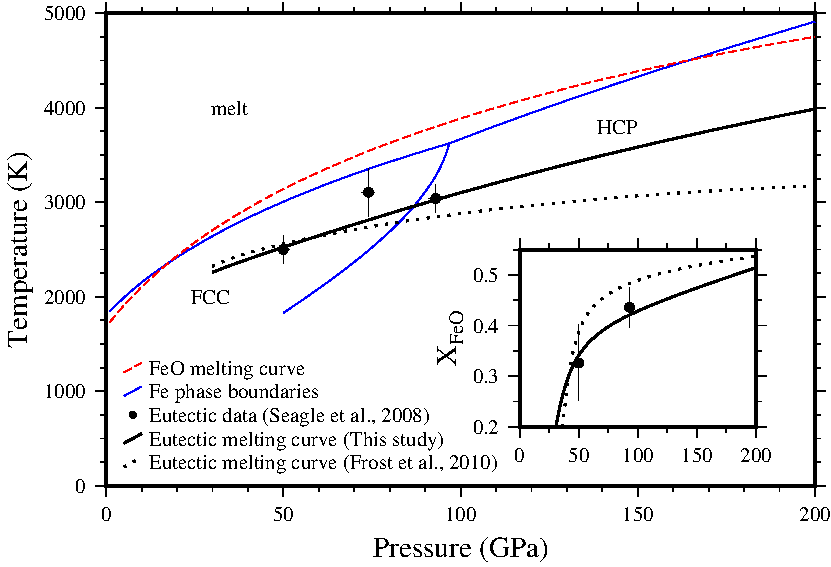
\includegraphics[width=0.8\textwidth]{figures/Fe_FeO_T_X_eutectic}
  \caption{Melting temperature in the Fe-O system as a function of pressure. Inset: eutectic composition in the Fe-O system.}
  \label{fig:Fe_O_melting}
\end{figure}




\section{Conclusions}

\cite{DKS2013}

\clearpage
\section*{References}

\bibliography{references_xs}

\end{document}
